\documentclass[journal]{IEEEtran}
\usepackage{cite}
\usepackage{amsmath,amssymb,amsfonts}
\usepackage{booktabs}
\usepackage{longtable}
\usepackage{graphicx}
\usepackage{url}
\makeatletter
\g@addto@macro{\UrlBreaks}{\do\/\do\_\do\-}
\makeatother
\usepackage{microtype}
\usepackage{flushend}

\begin{document}

\title{A 10{,}240-Byte Generator, Scored After It Is Selected}

\author{The DOPE Project}

\markboth{The DOPE Project}%
{A 10,240-Byte Generator}

\maketitle

\begin{abstract}
DOPE's measured generator on this panel is a compact residual network:
at most 12 inputs, one hidden layer of width 16 with $\tanh$ units, and a
refit linear readout. AdamW trains the hidden basis for 2{,}048 steps at
learning rate $0.002$. The shipped network has no embedding layer.
Each method is selected on its own objective. The shared measurements are
null-normalized retention at four times the fit size, and the bytes charged
to the artifact. On 97 informative PMLB regression lineages, the displayed
DOPE profile has median CatBoost retention $0.939876$ against $0.655681$
for a native-selected Gaussian copula, $0.585986$ for a study Chow--Liu
tree, and $-0.011971$ for study independent marginals. Ninety-eight of 100
DOPE artifacts are within the 10{,}240-byte cap; 62, 31, and 94 of the three
comparators are. A separate 21-lineage block compares DOPE with native-selected
CTGAN and TVAE. Every successful CTGAN and TVAE artifact in that ledger
exceeds the cap. Master Fitness v2 stays null: the six components and the
hard-gate map are not all present. Official tests remain sealed. No paired
superiority claim is made. Appendix~\ref{app:2048} lists every one of the 100
lineages. A separate 8{,}192-step budget on the same partitions is reported
in Appendix~\ref{app:8192} and is not adopted as the displayed model.
BeyondArena is a separate 142-family corpus in the dataset bucket. It is not
pooled with these 100 lineages. Five of twelve locked families were fit.
Seven did not prepare, and none of the five has a retention score.
\end{abstract}

\begin{IEEEkeywords}
Synthetic tabular data, compact generator, retention, artifact bytes.
\end{IEEEkeywords}

\section{Introduction}
A generator paper usually reports the metric that was also used to pick the
configuration. CTGAN and TVAE were introduced with a conditional generator
and a variational autoencoder, and later libraries score them with downstream
predictive efficacy~\cite{xu2019ctgan}. The Synthetic Data Vault fits
Gaussian-copula models inside that family~\cite{patki2016sdv}. Adversarial
random forests select a density through their forest density
estimator~\cite{watson2023arf}. Diffusion and CART synthesizers bring other
objectives~\cite{kotelnikov2023tabddpm,nowok2016synthpop}. Those native numbers
live on different scales.

The comparison here separates selection from the common measurement. DOPE,
the Gaussian copula, CTGAN, and TVAE keep the objectives published for those
methods. Chow--Liu and independent marginals are study implementations of the
published ideas, not the authors' packages~\cite{chow1968dependence}. After
selection, every retained artifact is measured by the same retention formula
and by the bytes required to sample from it. The pre-registered common scalar,
Master Fitness v2 (MFS-v2), is defined in Section~\ref{sec:scores}. It is
emitted only when every hard gate passes. On this panel the scalar is null
for every method.

The decision the measurements can support is narrower than ``which generator
is best.'' It is whether a network small enough to ship under a 10{,}240-byte
cap still preserves downstream regression utility on real validation rows.
Fig.~\ref{fig:bytes} is that comparison. TabDDPM and synthpop CART are cited
and have not been run on this panel. An unexecuted method is not a win for
DOPE.

\section{The network that was trained}
\label{sec:model}
The displayed profile is \path{features12_steps2048}. It is a compact neural
residual, not a GAN, a diffusion model, or a transformer. The training code
selects at most 12 screened inputs. A hidden layer of width 16 maps those
inputs through $\tanh$. AdamW, learning rate $0.002$, runs for 2{,}048 steps
on the regression mean-squared error, with gradient clipping at $5$. The
hidden weights and biases from that fit are kept. The intercept, the linear
skip coefficients, and the hidden readout are then refit by the same
regularized solver used for the native linear candidates, on the frozen
$\tanh$ features. Coefficients whose absolute value is below $10^{-5}$ are
dropped from the skip. For a selected input vector $x_S$ the shipped predictor is
\begin{equation}
\label{eq:residual}
h_j = \tanh\!\left(b_j + w_j^{\top} x_S\right),
\quad
\hat{y} = a + \beta^{\top} x_S + v^{\top} h .
\end{equation}
Sampling adds the noise model stored in the artifact. The codec accepts
hidden width 8 or 16 at the input counts used here and rejects widths 0, 17,
and 32. There is no embedding table in \eqref{eq:residual}. A separate
dataset-action router uses a vector of dimension
$856 + 24\times(128+10) = 4{,}168$. That vector does not generate the rows
in this paper.

The profile is a pre-registered reference. Compile-time search records the
proxy $0.45u + 0.25d + 0.30j$ and then keeps the candidate with the smallest
normalized gate shortfall, then the smallest artifact, then the lowest
candidate id. Every such compile is marked
\path{production_evidence_unmeasured}. No global DOPE family has been
selected, so the shared retention below was not allowed to choose the profile.

Other DOPE shapes exist and are not this result. Micro-TVAEs use latent and
hidden widths $4/16$, $8/24$, and $12/32$. TinyMAT uses widths 16 and 24.
Joint TVAE, masked-transformer, and TabSyn candidates use latent width 32 and
hidden width 128. A direct-rank TabDDPM candidate is a research comparator
with no claim on the 10{,}240-byte tier. The published fits did not retain a
per-step loss series, so this paper does not show a training curve.

On six confirmation lineages, disjoint from the discovery set, two longer
profiles were already measured at $4n$. CatBoost median retention is
$0.939543$ for the reference above, $0.937693$ for a width-16 profile trained
for 8{,}192 steps, and $0.949384$ for a width-8 profile trained for 8{,}192
steps. That is a six-lineage ablation. It does not replace the reference.

\section{Two scores}
\label{sec:scores}
Let $L_{\mathrm{null}}$, $L_{\mathrm{real}}$, and $L_{\mathrm{synthetic}}$ be
the auditor's loss on real validation rows when that auditor is trained on a
null baseline, on real fit rows, and on synthetic rows. Retention is
\begin{equation}
\label{eq:retention}
\frac{L_{\mathrm{null}}-L_{\mathrm{synthetic}}}{L_{\mathrm{null}}-L_{\mathrm{real}}} .
\end{equation}
A value of $1$ means the synthetic-trained auditor matched the real-trained
auditor. A value above $1$ means it beat the real-trained auditor. A negative
value means it did worse than the null. The denominator is the real model's
improvement over the null; when that improvement is negligible the lineage is
not informative and is omitted from the median. The three auditors are
CatBoost~\cite{prokhorenkova2018catboost}, ordinary linear regression, and an
MLP. Each reported median is the median across lineages of the median of
three sample seeds.

MFS-v2 is a different object. With component $c_i\in[0,1]$, weight $w_i>0$,
$\epsilon=10^{-6}$, and $W=\sum_i w_i$,
\begin{equation}
\label{eq:mfs}
\mathrm{MFS\text{-}v2}
= 100\exp\!\left(\frac{1}{W}\sum_i w_i\ln(\epsilon+c_i)\right)
\end{equation}
when the hard-gate map is non-empty, every hard gate passed, and every
positive-weight component is finite and inside $[0,1]$. Otherwise the scalar
is null. The weights are utility transfer $0.30$, driver fidelity $0.20$,
distribution fidelity $0.20$, structure fidelity $0.15$, coverage realism
$0.10$, and compactness $0.05$. Privacy's soft weight is zero, so a privacy
failure removes the score through a gate and does not move \eqref{eq:mfs}
directly. Utility transfer inside \eqref{eq:mfs} is a clamped one-sided 95\%
lower bound on gold retention. It is not the median of \eqref{eq:retention}.
Compactness is $\mathrm{clamp}(1 - \mathrm{bytes}/10240,\, 0,\, 1)$. Crossing
10{,}240 bytes fails the byte gate, so the scalar stays null.

Table~\ref{tab:illustration} applies \eqref{eq:mfs} to six invented components
$(0.90, 0.80, 0.85, 0.70, 0.75, 0.95)$. The resulting $82.40$ is arithmetic,
not a measurement. The second row is the same components with the byte gate
failed. The implementation returns null. No artifact in this paper has a
measured MFS-v2 value.

\begin{table}[t]
\caption{Illustration of \eqref{eq:mfs}. These components are not measurements.}
\label{tab:illustration}
\centering
\scriptsize
\setlength{\tabcolsep}{3pt}
\begin{tabular}{@{}lc@{}}
\toprule
Gate map & Scalar \\
\midrule
All six gates passed & $82.40$ \\
Byte gate failed & null \\
\bottomrule
\end{tabular}
\end{table}

\section{Protocol}
The panel is the rights-cleared PMLB regression collection~\cite{olson2017pmlb,romano2021pmlb}.
Of 104 MIT-licensed entries, four were excluded because a source row appeared
in both the official training and official test partitions. The remaining 100
use a grouped 80/20 fit and validation cut of the official training rows, seed
1729. Fit tables contain 72 to 800 rows. They are catalog coresets. Worker
directories contain no official test file. Official tests stay sealed, and
final evaluation is not authorized.

Fit seed 11 and sample seeds 101, 211, and 307 are the population actually
measured. Sizes $n$ and $4n$ are both stored; the tables below are $4n$.
Native objectives are not ranked across methods. The Gaussian copula row is
Copulas 0.14.1 \texttt{Gaussian\-Multivariate}, selected by held-out mean log
density. CTGAN and TVAE are the author implementation, selected by the mean of
linear and MLP regression $R^{2}$ on validation rows~\cite{xu2019ctgan}. ARF's
author \texttt{arfpy} core has closed its FORDE log-density fits and has not
yet been sampled on this shared schedule~\cite{watson2023arf}. Chow--Liu uses
eight bins and Laplace smoothing $1.0$ in study code. Independent marginals
are a study reference with no author package.

\section{Retention and bytes}
\label{sec:results}
\begin{figure*}[t]
\centering
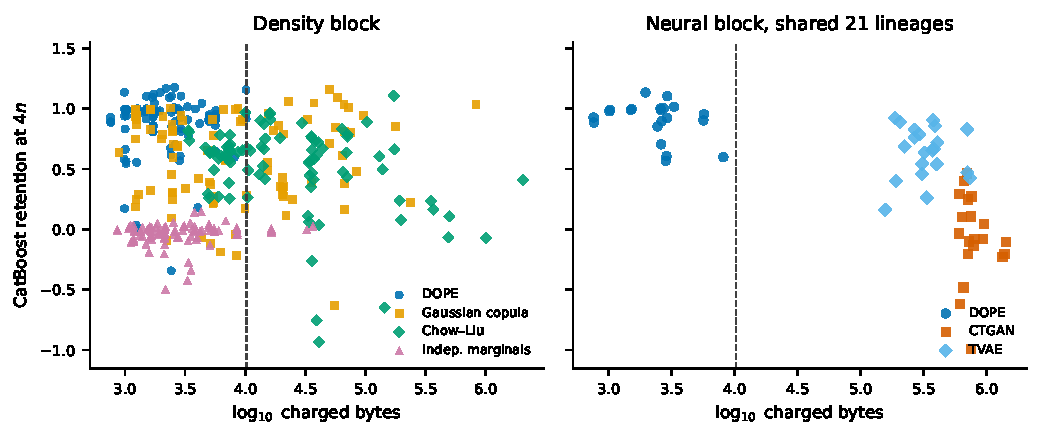
\includegraphics[width=0.98\textwidth]{figures/retention-bytes.pdf}
\caption{CatBoost retention at $4n$ against charged artifact bytes. The dashed
line is the 10{,}240-byte cap. The left panel is the density block. The right
panel is the 21 lineages on which native-selected CTGAN, native-selected TVAE,
and the DOPE reference all have an informative CatBoost median. The panels are
not one ranking.}
\label{fig:bytes}
\end{figure*}

Fig.~\ref{fig:bytes} plots one point per method and lineage. DOPE sits to the
left of the cap and near retention $1$. Independent marginals are also small
and sit near retention $0$. The Gaussian copula and the study Chow--Liu tree
spread across the cap. CTGAN and TVAE sit between about $10^{5}$ and
$10^{6}$ bytes.

Table~\ref{tab:density} is the paired density block. The CatBoost column
repeats the medians already published for this profile. Linear and MLP come
from the same paired records. The Gaussian copula is close to DOPE under the
linear auditor ($0.989300$ versus $0.994046$) and farther under CatBoost and
the MLP. The study tree and the independent marginals stay below DOPE on all
three auditors. Lineage counts differ because a lineage is omitted when that
auditor's real-versus-null gap is not informative. Median dataset-level
differences are positive and the pre-registered paired test has not been run,
so the comparison is inconclusive.

\begin{table}[t]
\caption{Density block at $4n$, fit seed 11. Medians of per-lineage
three-seed medians. Study code is marked.}
\label{tab:density}
\centering
\scriptsize
\setlength{\tabcolsep}{2.5pt}
\begin{tabular}{@{}llrrr@{}}
\toprule
Auditor & Comparator & $n$ & DOPE & Other \\
\midrule
CatBoost & Gaussian copula & 97 & 0.939876 & 0.655681 \\
CatBoost & Chow--Liu, study & 97 & 0.939876 & 0.585986 \\
CatBoost & Indep.\ marginals, study & 97 & 0.939876 & $-0.011971$ \\
Linear & Gaussian copula & 92 & 0.994046 & 0.989300 \\
Linear & Chow--Liu, study & 92 & 0.994046 & 0.661218 \\
Linear & Indep.\ marginals, study & 92 & 0.994046 & 0.002056 \\
MLP & Gaussian copula & 75 & 1.061123 & 0.927569 \\
MLP & Chow--Liu, study & 75 & 1.061123 & 0.691645 \\
MLP & Indep.\ marginals, study & 75 & 1.061123 & $-0.027881$ \\
\bottomrule
\end{tabular}
\end{table}

Table~\ref{tab:bytes} counts artifacts at or under 10{,}240 charged bytes.
Two of 100 DOPE artifacts exceed the cap (the largest is 22{,}233 bytes).
Independent marginals pass the cap more often than the Chow--Liu study tree
and still have retention near zero. Smallness alone is not the result.

\begin{table}[t]
\caption{Charged bytes at $4n$. Density methods use 100 lineages. CTGAN and
TVAE use the 22 native-selected artifacts that produced a size-$4$ sample,
which is a wider set than the 21 informative retention lineages.}
\label{tab:bytes}
\centering
\scriptsize
\setlength{\tabcolsep}{3pt}
\begin{tabular}{@{}lrr@{}}
\toprule
Method & Median bytes & Within cap \\
\midrule
DOPE reference & 1{,}895.5 & 98/100 \\
Gaussian copula & 5{,}464.5 & 62/100 \\
Chow--Liu, study & 29{,}865 & 31/100 \\
Indep.\ marginals, study & 2{,}549.5 & 94/100 \\
CTGAN & 741{,}834 & 0/22 \\
TVAE & 317{,}141.5 & 0/22 \\
\bottomrule
\end{tabular}
\end{table}

Table~\ref{tab:neural} is the neural block. It is not pooled with
Table~\ref{tab:density}. DOPE's CatBoost median on these 21 lineages is
$0.953366$, CTGAN's is $-0.081259$, and TVAE's is $0.669033$. The same
direction appears for the linear auditor and the MLP, on 21 and 19 lineages.
The ledger also records 525 scheduling cutoffs for the CTGAN/TVAE search.
Those cutoffs are unfinished work, not method failures, and they are why this
block cannot support a method-wide conclusion.

\begin{table}[!b]
\caption{Neural block at $4n$. CTGAN and TVAE are native-selected author
code. This lineage set is not the density block.}
\label{tab:neural}
\centering
\scriptsize
\setlength{\tabcolsep}{2.5pt}
\begin{tabular}{@{}llrrr@{}}
\toprule
Auditor & Comparator & $n$ & DOPE & Other \\
\midrule
CatBoost & CTGAN & 21 & 0.953366 & $-0.081259$ \\
CatBoost & TVAE & 21 & 0.953366 & 0.669033 \\
Linear & CTGAN & 21 & 0.998972 & $-0.033499$ \\
Linear & TVAE & 21 & 0.998972 & 0.795925 \\
MLP & CTGAN & 19 & 1.025597 & $-0.148653$ \\
MLP & TVAE & 19 & 1.025597 & 0.752792 \\
\bottomrule
\end{tabular}
\end{table}

\begin{samepage}
One shared lineage goes the other way. On \path{1193_BNG_lowbwt},
native-selected TVAE retention is $1.029$ at 293{,}868 bytes and the DOPE
reference is $0.970$ at 2{,}436 bytes. On \path{503_wind} the same DOPE
profile is $0.996$ at 3{,}846 bytes and TVAE is $0.802$ at 471{,}140 bytes.
\end{samepage}

\section{The common scalar}
Table~\ref{tab:score} is the MFS-v2 column required by Section~\ref{sec:scores}.
No method has a complete component vector and a fully passed hard-gate map on
this panel, so every scalar is null. Copying a retention number or a zero into
this column would publish a value the contract refuses to emit. PTF-v1 is
also null. Release-safe certification is null. The 100 lineages do not meet
the production requirement of at least 30 informative groups under the final
profile gate, and the five admission locks are not frozen.

\begin{table}[t]
\caption{MFS-v2 after native selection. Null means the scalar was not emitted.}
\label{tab:score}
\centering
\scriptsize
\begin{tabular}{@{}lc@{}}
\toprule
Method & MFS-v2 \\
\midrule
DOPE reference & null \\
Gaussian copula & null \\
CTGAN & null \\
TVAE & null \\
ARF & null \\
TabDDPM & null \\
synthpop CART & null \\
Chow--Liu, study code & null \\
Indep.\ marginals, study code & null \\
\bottomrule
\end{tabular}
\end{table}

\section{Every lineage, not only the median}
\label{sec:every}
Table~\ref{tab:density} is the median of Appendix~\ref{app:2048}. That appendix
has one row for each of the 100 rights-cleared lineages: the PMLB name, the
fit-row count, the feature count, the size-$4n$ byte charge, the L3 flag, and
the three-seed median retention at $n$ and at $4n$. A blank cell is an
unavailable fit or an auditor that is not informative on all three sample
seeds. It is not a zero. Two displayed-profile fits are unavailable,
\path{4544_GeographicalOriginalofMusic} and \path{588_fri_c4_1000_100}.
\path{678_visualizing_environmental} has a fit whose CatBoost group is not
informative on all three seeds. The CatBoost median therefore uses 97
lineages, and the byte count uses 100.

Fig.~\ref{fig:every} plots those medians against charged bytes for CatBoost.
The same drawing for the linear auditor and the MLP is in the figure
directory. The frame is $[-1.5, 1.6]$. Points outside it remain in the
appendix; the panel title counts them. The dashed line is $\log_{10}(10240)$.
Fig.~\ref{fig:pairs} is the paired difference, displayed profile minus each
native-selected density comparator, with the lineage name on the axis. The
frame is $[-1.5, 1.5]$ for the same reason. These figures are descriptive.
They are not a paired superiority test.

\begin{figure*}[t]
\centering
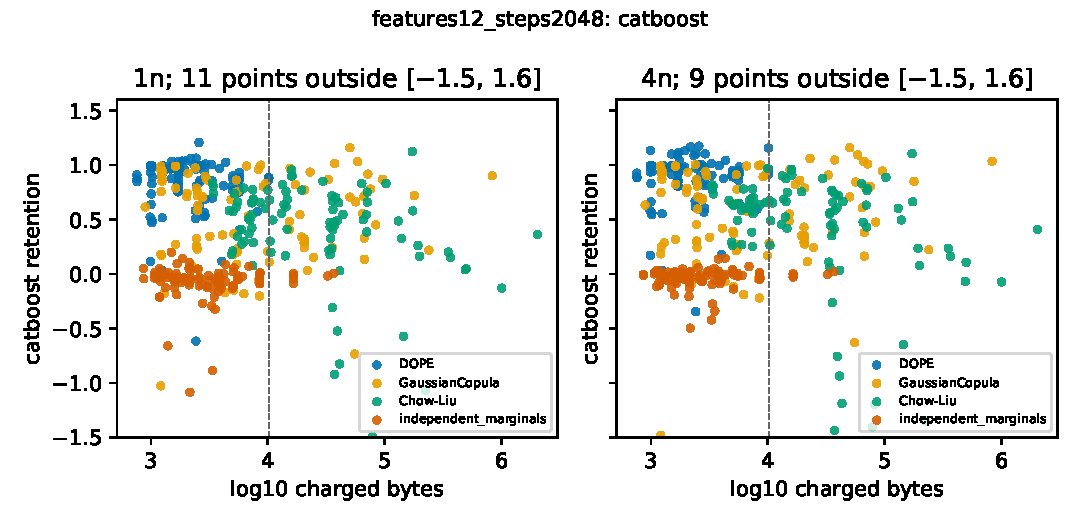
\includegraphics[width=\textwidth]{figures/s3-retention-bytes-catboost.pdf}
\caption{CatBoost retention against charged bytes for every informative
lineage of \texttt{features12\_steps2048} and the native-selected density
comparators. The neural block is not on this figure.}
\label{fig:every}
\end{figure*}

\begin{figure*}[t]
\centering
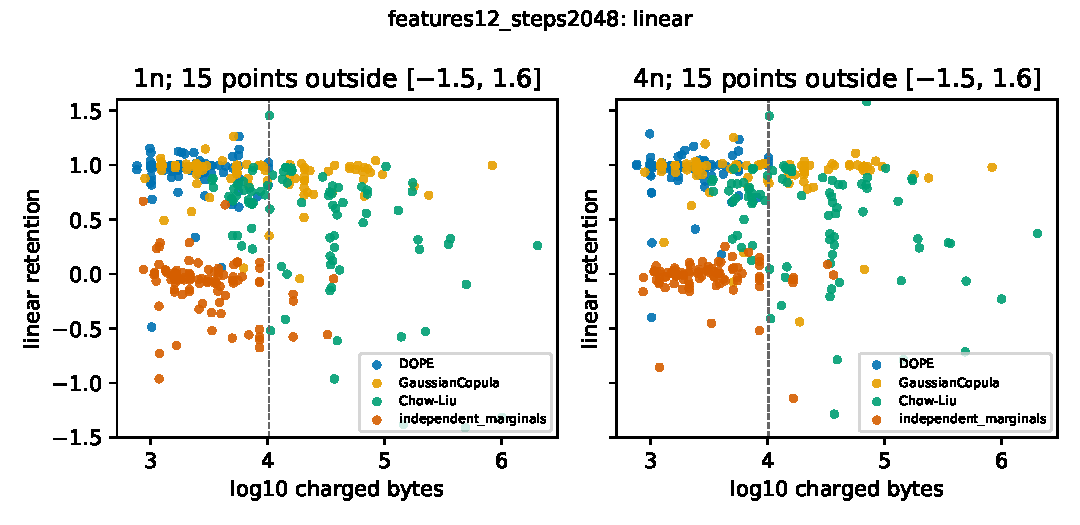
\includegraphics[width=\textwidth]{figures/s3-retention-bytes-linear.pdf}
\caption{Linear retention against charged bytes, same lineages and frame as
Fig.~\ref{fig:every}.}
\label{fig:linear}
\end{figure*}

\begin{figure*}[t]
\centering
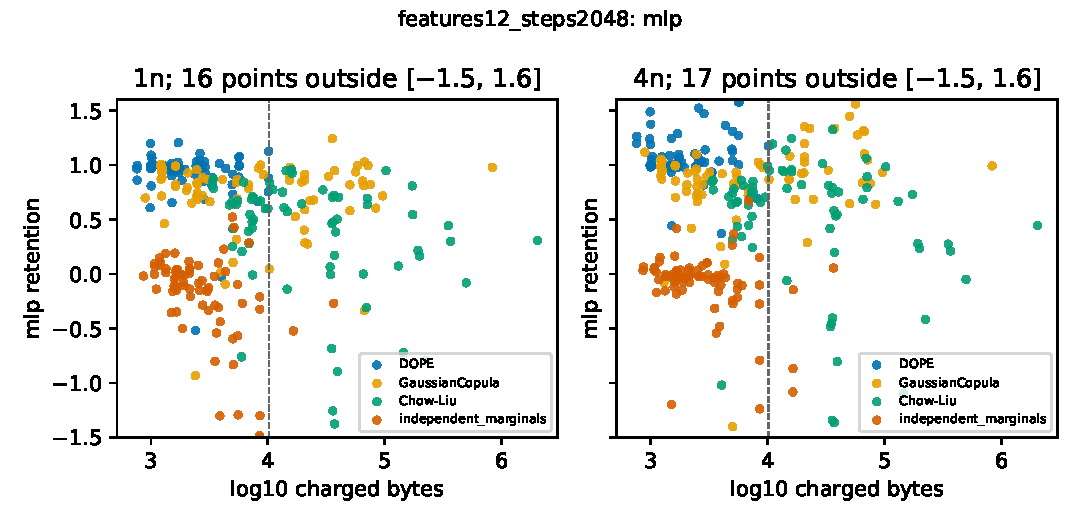
\includegraphics[width=\textwidth]{figures/s3-retention-bytes-mlp.pdf}
\caption{MLP retention against charged bytes, same lineages and frame as
Fig.~\ref{fig:every}.}
\label{fig:mlp}
\end{figure*}

\begin{figure*}[t]
\centering
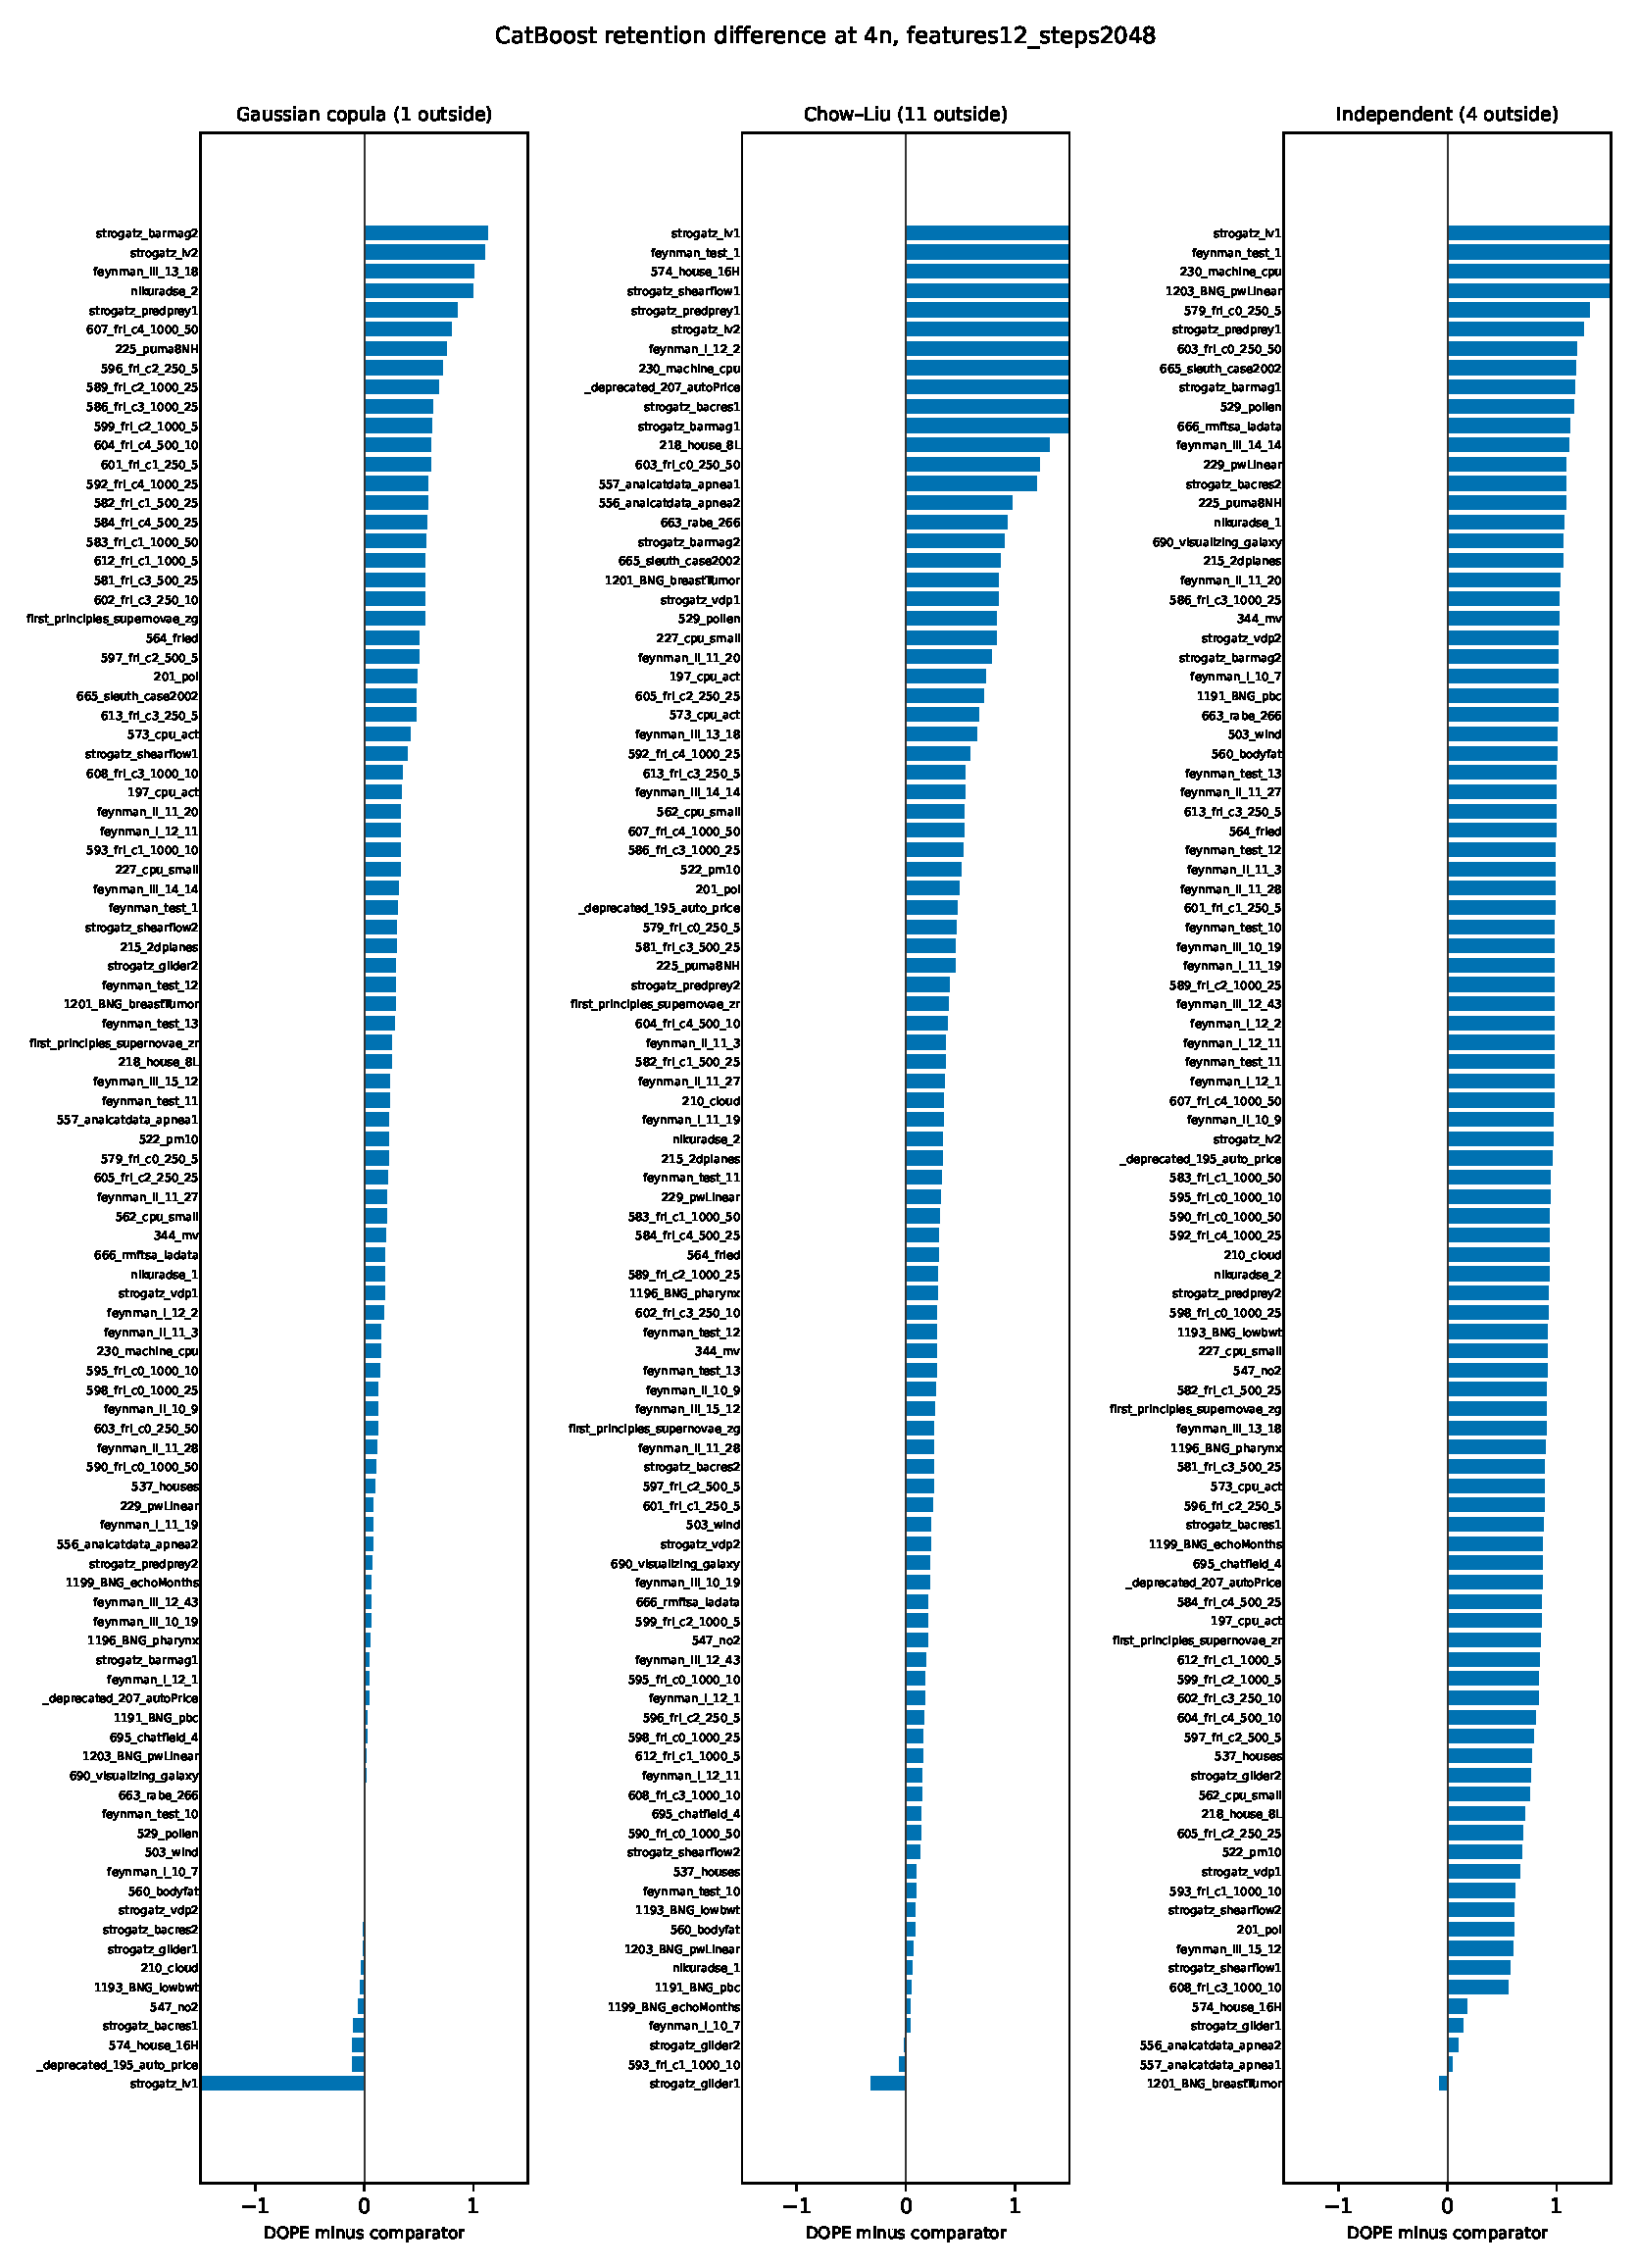
\includegraphics[width=\textwidth,height=0.92\textheight,keepaspectratio]{figures/s3-paired-differences.pdf}
\caption{Paired CatBoost difference at $4n$. Each bar is one informative
lineage. Differences outside $[-1.5, 1.5]$ are counted in the panel title
and listed in Appendix~\ref{app:2048}.}
\label{fig:pairs}
\end{figure*}

\section{Eight thousand steps on the same partitions}
\label{sec:steps}
\path{features12_steps8192} is the same residual with four times as many
AdamW steps. It was already fit in the closed expansion round. Of the 100
lineages, 68 have a successful fit. Thirty failed before the fit started
because of transport or prelaunch, one failed because a foreign GPU owner
appeared, and one failed the charged-artifact cap. Sample evaluation of that
round has 408 measured cells and 192 fit-unavailable cells for this profile.
Sixty-eight of the 69 artifacts with a byte charge are within 10{,}240 bytes.
The largest charged artifact is 19{,}041 bytes.

On the lineages where both budgets have a complete three-seed group, the
CatBoost medians are $0.925519$ at 2{,}048 steps and $0.970348$ at 8{,}192
steps (68 lineages; median paired difference $0.034349$). The linear medians
are $0.990163$ and $0.986519$ (64 lineages; median paired difference
$-0.000283$). The MLP medians are $1.065260$ and $1.056573$ (52 lineages;
median paired difference $0.004514$). The extra steps are a budget check.
They do not replace \path{features12_steps2048} as the displayed model, and
they are not a superiority test. Appendix~\ref{app:8192} lists all 100.

The scored fits did not retain a per-step loss. A logged replay of both
budgets, written to a new directory and not substituted for those artifacts,
records the AdamW training loss and the training-derived validation loss at
every step. The curves are the hidden-basis objective, before the closed-form
readout refit. All 100 lineages finished both budgets, and every recorded
loss is finite. The median training loss starts at $0.321246$. It ends at
$0.002745$ after 2{,}048 steps and at $0.000763$ after 8{,}192 steps. The
median validation loss starts at $0.270883$ and ends at $0.004433$ and
$0.001813$. Figure~\ref{fig:loss2048} and Figure~\ref{fig:loss8192} draw the
median and the band from the 10th to the 90th percentile. \path{losses.png}
is not that series. The lower hidden-basis loss at 8{,}192 steps does not
replace the displayed profile.

\begin{figure*}[t]
\centering
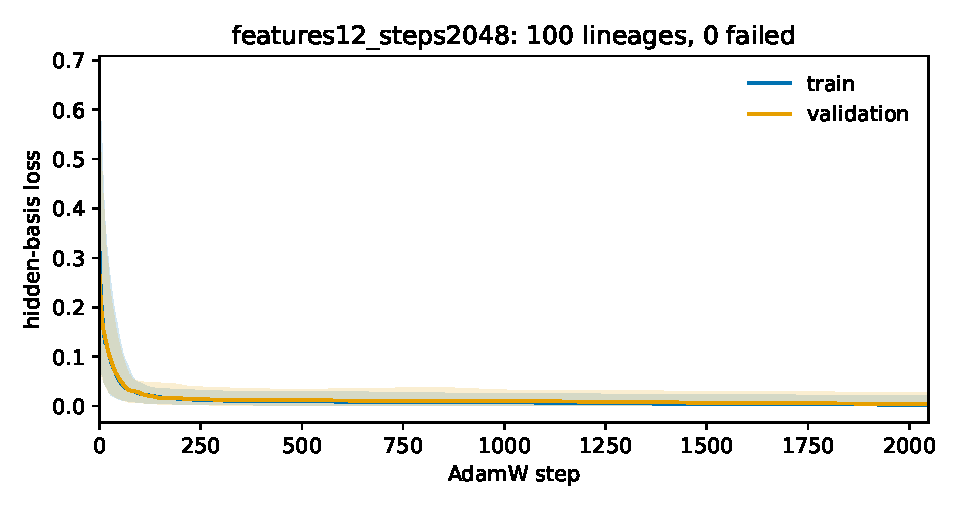
\includegraphics[width=0.82\textwidth]{figures/s3-loss-steps2048.pdf}
\caption{AdamW hidden-basis loss at 2{,}048 steps. The line is the median of 100 lineages. The band is the 10th to the 90th percentile, before the readout refit.}
\label{fig:loss2048}
\end{figure*}

\begin{figure*}[t]
\centering
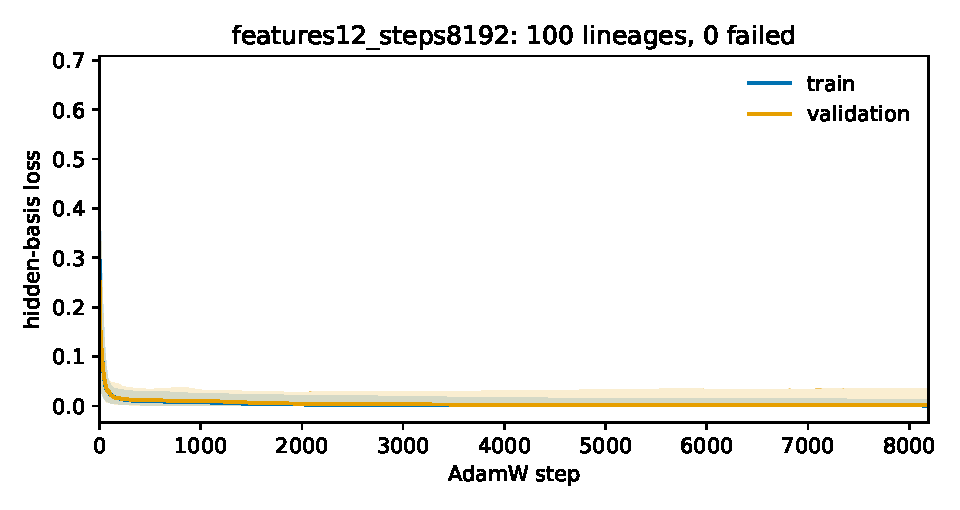
\includegraphics[width=0.82\textwidth]{figures/s3-loss-steps8192.pdf}
\caption{AdamW hidden-basis loss at 8{,}192 steps, same 100 lineages and same band. This budget is not the displayed model.}
\label{fig:loss8192}
\end{figure*}

\section{BeyondArena is a separate corpus}
\label{sec:beyond}
{\raggedright
BeyondArena is the pinned TabArena/BeyondArena snapshot
\path{2ecfe882ccfb814fc27c4de10a64ceefd5d7655c} in
\path{s3://veox-jopedime-datasets-use2/benchmarks/BeyondArena/}.\par}
The index lists 142 source families, 19{,}676{,}576 rows, and 3{,}722 official
folds. The task mix is 73 binary, 44 regression, and 25 multiclass. The split
regimes are 103 IID, 21 temporal, and 18 grouped. Every family is stored once
under \path{raw/BeyondArena/} at that revision. The research prefix
\path{research/BeyondArena/} holds later experiment handoffs, not a second copy
of the tables. Appendix~\ref{app:beyond} names all 142.

The fit lock takes at most 12 binary or regression families whose recorded
license is a redistribution grant, labels each with the published split
regime, and round-robins IID, grouped, and temporal in hash order of the
source-family id. Multiclass families and licenses without that grant stay
out. None of the 12 is one of the 100 PMLB lineages.
{\raggedright
The locked names are
\path{airfoil_self_noise},
\path{early_learning_predictors},
\path{lending_club},
\path{heart_disease_va_long_beach},
\path{musk},
\path{kick},
\path{qsar_biodeg},
\path{telemonitoring_parkinsons_biomedical_voice_measurements},
\path{hotel_booking_demand},
\path{wine_world_cost},
\path{video_transcoding_time_prediction},
and \path{garments_worker_productivity}.\par}
Official fold 0 of repeat 0 is the fit source. An 80/20 grouped cut of that
official training fold, seed 1729, supplies the fit and the validation loss.
The official test rows stay in the evaluator directory. Four families,
\path{early_learning_predictors}, \path{lending_club}, \path{kick}, and
\path{wine_world_cost}, exceed the 2{,}000-feature projection cap.
\path{lending_club} still does after 14 all-missing training columns are
dropped. \path{heart_disease_va_long_beach}, \path{qsar_biodeg}, and
\path{hotel_booking_demand} have an identical source row on both sides of the
official fold, the same overlap rule that excluded four PMLB lineages.
The other five families completed both budgets. Every artifact is inside the
10{,}240-byte cap. Table~\ref{tab:beyond} records the charged bytes and the
final hidden-basis validation loss. No retention auditor was run on this
block, so it has no retention column, and it is not pooled with the 100 or
with the 21-lineage neural block. \eqref{eq:mfs} stays null.

\begin{table}[t]
\caption{BeyondArena families that prepared. Bytes are the charged artifact. The loss is the final AdamW hidden-basis validation loss, before the readout refit.}
\label{tab:beyond}
\centering
\scriptsize
\setlength{\tabcolsep}{3.2pt}
\begin{tabular}{@{}lrrrrr@{}}
\toprule
family & fit rows & 2{,}048 B & 8{,}192 B & val 2{,}048 & val 8{,}192\\
\midrule
airfoil\_self\_noise & 802 & 804 & 818 & 0.0101 & 0.0045\\
musk & 3{,}738 & 9{,}273 & 9{,}350 & 0.1456 & 0.0903\\
telemonitoring & 257 & 1{,}852 & 1{,}890 & 0.0333 & 0.0190\\
video\_transcoding & 35{,}918 & 5{,}054 & 5{,}071 & 0.0025 & 0.0020\\
garments\_productivity & 939 & 2{,}317 & 2{,}372 & 0.0277 & 0.0251\\
\bottomrule
\end{tabular}
\normalsize
\end{table}

\section{What this panel does not establish}
The fits use coresets of 72--800 rows, one fit seed, and a training-derived
validation cut. They do not establish behavior on the full tables used by
TabDDPM, a five-seed campaign, production PTF-v1, or a release decision.
ARF sampling and the TabDDPM run on these 100 lineages are still ahead.
A closed refinement-validation round accounts for 1{,}200 logical cells, 816
measured and 384 unavailable, and it likewise leaves \eqref{eq:mfs} null.
Its public report is not yet issued: each measured sample directory contains
two unlisted scratch directories, so the receipt inventory check fails closed.
Nothing in that failure opens an official test or assigns a fitness score.

When a later round measures the six components, Table~\ref{tab:score} is the
column to fill, and only through the implementation of \eqref{eq:mfs}. A
paired interval can be added only after the protocol's paired test is
computed. Until then the public statement is the one in the abstract: the
residual is specified, retention and bytes are measured on the blocks above,
and the common scalar is null.

\section*{Ledger}
The medians, lineage counts, byte ranges, and null flags are the 5 October
2026 entries in \path{research/benchmark/RESULTS_STATUS.md}, taken from the
density-matched and SDV-matched population validation files and from
\path{research/benchmark/results/s3-lineage-record.json}. Fitness weights are
\path{production/kpi-contract.json}. The displayed profile remains
\path{features12_steps2048}.

\onecolumn
\appendices
\section{Displayed profile, all 100 lineages}
\label{app:2048}
\footnotesize
\begin{longtable}{llllllllll}
\caption{Displayed profile, all 100 lineages. The cap column is charged bytes at or under 10{,}240. It is not a release certificate.}\\
\toprule
id & name & rows & feat. & bytes & cap & CB $n$ & CB $4n$ & lin $4n$ & MLP $4n$\\
\midrule
\endfirsthead
\toprule
id & name & rows & feat. & bytes & cap & CB $n$ & CB $4n$ & lin $4n$ & MLP $4n$\\
\midrule
\endhead
\bottomrule
\endfoot
02a45777900441ce & 215\_2dplanes & 800 & 10 & 2,583 & pass & 0.9930 & 1.0001 & 0.9990 & 1.0477\\
047e62b52a3f4ede & 695\_chatfield\_4 & 156 & 12 & 3,311 & pass & 1.0041 & 1.0155 & 1.0048 & ---\\
04c80944e971cb3e & first\_principles\_supernovae\_zr & 157 & 1 & 762 & pass & 0.8753 & 0.8846 & 0.9959 & 1.2627\\
0561d673cb73c27e & 666\_rmftsa\_ladata & 339 & 10 & 2,921 & pass & 1.0095 & 1.1026 & 1.0338 & 1.1394\\
060b9fff8092db17 & 589\_fri\_c2\_1000\_25 & 667 & 25 & 5,717 & pass & 0.8893 & 0.9534 & 0.9911 & 1.5794\\
06b0312a585b436e & 1196\_BNG\_pharynx & 800 & 10 & 2,631 & pass & 0.8601 & 0.8964 & 1.0458 & 1.7049\\
0779d3fd5b3133a2 & nikuradse\_2 & 241 & 1 & 758 & pass & 0.9096 & 0.9261 & 2.1723 & 2.2082\\
07f38946316c039b & 593\_fri\_c1\_1000\_10 & 667 & 10 & 2,876 & pass & 0.5650 & 0.6068 & 0.9617 & 1.6005\\
0a8428ef25a69175 & 537\_houses & 800 & 8 & 2,609 & pass & 0.6257 & 0.7036 & 1.0150 & 1.0256\\
0d482c1dd7cc6592 & 210\_cloud & 72 & 5 & 1,844 & pass & 1.0374 & 0.9772 & 1.0944 & 1.0239\\
0db59fd2579600d0 & 665\_sleuth\_case2002 & 98 & 6 & 1,962 & pass & 1.0371 & 1.1324 & 1.1345 & ---\\
0f86a714ec5f3ac6 & 1191\_BNG\_pbc & 800 & 18 & 4,183 & pass & 0.8097 & 0.8761 & 0.9173 & ---\\
167578f5deba4977 & 547\_no2 & 333 & 7 & 2,443 & pass & 0.8073 & 0.8513 & 1.0097 & 0.9898\\
19f2c3c2d67defd7 & feynman\_II\_11\_27 & 800 & 4 & 1,494 & pass & 0.9704 & 0.9890 & 0.9960 & 1.0048\\
19f4780b53b3fa41 & 678\_visualizing\_environmental & 74 & 3 & 1,515 & pass & --- & --- & --- & 0.4431\\
1a4456d1cc71a26a & feynman\_test\_1 & 800 & 7 & 2,191 & pass & 1.0608 & 1.1671 & 0.9816 & ---\\
1a803b27c2400dc4 & feynman\_III\_10\_19 & 800 & 4 & 1,520 & pass & 0.9882 & 0.9952 & 0.9942 & 0.9965\\
1cb97b1d7314d43d & 229\_pwLinear & 133 & 10 & 2,587 & pass & 0.8417 & 0.9878 & 0.9104 & ---\\
205f4b4982b9ea49 & 608\_fri\_c3\_1000\_10 & 667 & 10 & 2,845 & pass & 0.5263 & 0.5671 & 1.0451 & 0.8182\\
26eff843be35d831 & 581\_fri\_c3\_500\_25 & 333 & 25 & 5,647 & pass & 0.7602 & 0.9020 & 1.1297 & 1.5792\\
282f8ddb43b5e677 & 595\_fri\_c0\_1000\_10 & 667 & 10 & 2,904 & pass & 0.8974 & 0.9234 & 0.9962 & 1.0250\\
297b7688a045c583 & 603\_fri\_c0\_250\_50 & 167 & 50 & 10,171 & pass & 0.8848 & 1.1562 & 1.0700 & 2.6883\\
2c8d0985f3557d2b & feynman\_II\_11\_28 & 800 & 2 & 1,026 & pass & 0.9831 & 0.9899 & 1.0031 & 0.9976\\
30ca2887550f0d8d & 201\_pol & 800 & 26 & 8,145 & pass & 0.5742 & 0.5976 & 0.7015 & 0.6923\\
3408a6a513c627a3 & strogatz\_barmag1 & 267 & 2 & 1,011 & pass & 0.9750 & 0.9775 & 0.9969 & 1.0058\\
35a9aa9b88f0e4d1 & 344\_mv & 800 & 10 & 2,737 & pass & 0.9985 & 1.0016 & 0.9662 & 1.0347\\
3d3321e27d14f9aa & 599\_fri\_c2\_1000\_5 & 667 & 5 & 1,707 & pass & 0.8359 & 0.8611 & 0.9668 & 1.6797\\
44eaabe4cb923766 & 613\_fri\_c3\_250\_5 & 167 & 5 & 1,712 & pass & 0.8671 & 0.9276 & 0.8599 & ---\\
46b25db9396c8209 & 227\_cpu\_small & 800 & 12 & 3,327 & pass & 0.8569 & 0.9072 & 0.9018 & 0.9364\\
46c5a59e5ae42037 & 1193\_BNG\_lowbwt & 800 & 9 & 2,436 & pass & 0.9635 & 0.9703 & 1.0030 & 0.9871\\
471f11cc2d38853a & feynman\_test\_11 & 800 & 4 & 1,481 & pass & 0.9645 & 0.9760 & 0.9975 & 0.9826\\
47c581af5de1136b & 582\_fri\_c1\_500\_25 & 333 & 25 & 5,670 & pass & 0.7510 & 0.9088 & 0.7173 & ---\\
48b7a3bf81e5f3e5 & 605\_fri\_c2\_250\_25 & 167 & 25 & 5,692 & pass & 0.4046 & 0.6465 & 1.9138 & ---\\
4a354d98c965b01f & 597\_fri\_c2\_500\_5 & 333 & 5 & 1,713 & pass & 0.7550 & 0.8055 & 0.9814 & 1.8381\\
4aa84fff8ad0cd26 & feynman\_III\_13\_18 & 800 & 4 & 1,501 & pass & 0.8748 & 0.9137 & 0.8850 & 0.9348\\
51730b348b1bbd14 & 557\_analcatdata\_apnea1 & 316 & 3 & 1,237 & pass & -0.0032 & 0.0086 & --- & ---\\
54b221668673164c & feynman\_III\_14\_14 & 800 & 5 & 1,726 & pass & 1.0346 & 1.1164 & 1.0011 & 1.0611\\
552665868f8f72ed & strogatz\_vdp2 & 267 & 2 & 989 & pass & 0.9945 & 0.9963 & 0.9960 & 0.9969\\
585fef2a1cb6b33f & strogatz\_lv2 & 267 & 2 & 1,018 & pass & 0.8286 & 0.9859 & 0.7502 & ---\\
642738a361f1c63a & feynman\_I\_12\_1 & 800 & 2 & 1,032 & pass & 0.9892 & 0.9910 & 0.9892 & 0.9933\\
64c64f0f9983c48f & strogatz\_bacres2 & 267 & 2 & 998 & pass & 0.9793 & 0.9832 & 0.9783 & 0.9862\\
654566a1f91408aa & 4544\_GeographicalOriginalofMusic & 706 & 117 & 22,233 & fail & --- & --- & --- & ---\\
693890aae9dc860b & first\_principles\_supernovae\_zg & 162 & 1 & 761 & pass & 0.8492 & 0.8908 & 1.0066 & 1.1997\\
6cacb11611345a24 & feynman\_I\_11\_19 & 800 & 6 & 1,947 & pass & 0.9524 & 0.9812 & 0.9780 & 0.9800\\
7291b347fe0238fb & feynman\_II\_11\_20 & 800 & 5 & 1,757 & pass & 0.9928 & 1.0432 & 1.0016 & 1.0674\\
7423783f7e38bb9b & strogatz\_shearflow1 & 267 & 2 & 1,021 & pass & 0.4900 & 0.5614 & -0.3978 & ---\\
7a3d123dd555110d & 598\_fri\_c0\_1000\_25 & 667 & 25 & 5,668 & pass & 0.8613 & 0.9166 & 1.0046 & 1.0034\\
7c8943b160464add & 601\_fri\_c1\_250\_5 & 167 & 5 & 1,719 & pass & 0.7859 & 0.8552 & 1.0773 & ---\\
7e51711baa1b1fb1 & feynman\_I\_12\_11 & 800 & 5 & 1,718 & pass & 0.9267 & 0.9320 & 1.0015 & 0.9860\\
80589368fa78f21a & 218\_house\_8L & 800 & 8 & 2,392 & pass & 0.5835 & 0.6708 & 0.9616 & 1.1040\\
8164950b155f7f56 & feynman\_I\_12\_2 & 800 & 4 & 1,511 & pass & 0.9702 & 0.9986 & 0.9485 & 0.9753\\
85a31ae409944a1b & feynman\_II\_10\_9 & 800 & 3 & 1,269 & pass & 0.9330 & 0.9508 & 0.9589 & 0.9515\\
8d859cfa7b51a351 & feynman\_III\_15\_12 & 800 & 3 & 1,248 & pass & 0.5172 & 0.5542 & 1.0228 & 1.0749\\
923483635406b213 & 1203\_BNG\_pwLinear & 800 & 10 & 2,581 & pass & 1.2079 & 1.1750 & 0.9941 & 1.5230\\
9312d813229df035 & 690\_visualizing\_galaxy & 216 & 4 & 1,458 & pass & 0.9725 & 0.9755 & 0.9853 & 1.0870\\
94a00ea67f49bf84 & 596\_fri\_c2\_250\_5 & 167 & 5 & 1,698 & pass & 0.7546 & 0.8072 & --- & ---\\
94bd4520b8ceb3f0 & feynman\_test\_12 & 800 & 5 & 1,747 & pass & 0.9688 & 0.9804 & 0.9913 & 1.0067\\
956d34f13e7af830 & 586\_fri\_c3\_1000\_25 & 667 & 25 & 5,701 & pass & 0.9325 & 0.9849 & 1.2339 & 2.1457\\
9a10c15885022034 & \_deprecated\_195\_auto\_price & 106 & 15 & 5,025 & pass & 0.8717 & 0.9485 & 0.9598 & 1.3107\\
a04f964bc53281e0 & strogatz\_lv1 & 267 & 2 & 985 & pass & -3.8784 & -3.4212 & --- & ---\\
a23f4bd626b76590 & feynman\_test\_13 & 800 & 5 & 1,740 & pass & 0.9178 & 0.9605 & 0.9900 & 1.0991\\
a32a69e7c701eb14 & 588\_fri\_c4\_1000\_100 & 667 & 100 & 19,019 & fail & --- & --- & --- & ---\\
a5ba682572f53add & 602\_fri\_c3\_250\_10 & 167 & 10 & 2,900 & pass & 0.5355 & 0.8109 & 0.7988 & ---\\
a863cd42be4d05d4 & 663\_rabe\_266 & 80 & 2 & 1,014 & pass & 0.9781 & 0.9933 & 0.9967 & 1.0521\\
a97065df07a47eb0 & 592\_fri\_c4\_1000\_25 & 667 & 25 & 5,655 & pass & 0.8791 & 0.9340 & 0.9578 & 1.2714\\
ab279eded3b3c52b & 574\_house\_16H & 800 & 16 & 4,035 & pass & 0.1181 & 0.1796 & 0.1795 & 0.3705\\
aebf5d861a8365b4 & 522\_pm10 & 333 & 7 & 2,409 & pass & 0.5082 & 0.6149 & 0.4125 & 2.3076\\
b6adf79118a58cea & 562\_cpu\_small & 800 & 12 & 3,353 & pass & 0.6968 & 0.7747 & 0.9834 & 0.9307\\
b78d323566930bd7 & 583\_fri\_c1\_1000\_50 & 667 & 50 & 10,098 & pass & 0.8607 & 0.9444 & 0.9960 & 1.6211\\
b7f9774e2142a758 & strogatz\_shearflow2 & 267 & 2 & 1,019 & pass & 0.4707 & 0.5439 & 0.7450 & 1.8955\\
bc85856c012bcc1b & 607\_fri\_c4\_1000\_50 & 667 & 50 & 10,209 & pass & 0.8856 & 0.9640 & 3.9394 & ---\\
c107ee39eb333a9d & 584\_fri\_c4\_500\_25 & 333 & 25 & 5,638 & pass & 0.8062 & 0.8619 & 0.9417 & ---\\
c30ff9405c916718 & 579\_fri\_c0\_250\_5 & 167 & 5 & 1,692 & pass & 0.9475 & 1.0923 & 0.9961 & 0.9783\\
c4f8e81b70d33a13 & 590\_fri\_c0\_1000\_50 & 667 & 50 & 10,180 & pass & 0.8839 & 0.9172 & 1.0359 & 1.1762\\
c649a4cee87c4321 & 529\_pollen & 800 & 4 & 1,506 & pass & 1.0356 & 1.1012 & 0.9717 & 1.2459\\
cb5bf66ef2ee09ed & nikuradse\_1 & 241 & 2 & 992 & pass & 0.9346 & 0.9373 & 0.9997 & 1.1909\\
cba8393879afd1dc & 230\_machine\_cpu & 140 & 6 & 2,338 & pass & 1.0026 & 1.0891 & 1.1718 & ---\\
ce1a79e2d658eb8a & strogatz\_glider2 & 267 & 2 & 1,003 & pass & 0.6382 & 0.6625 & 1.0720 & 1.3756\\
ce837ccd24a3a18c & strogatz\_bacres1 & 267 & 2 & 1,004 & pass & 0.7352 & 0.8309 & 0.9014 & 0.9826\\
cee6f811d0bf199d & feynman\_II\_11\_3 & 800 & 5 & 1,728 & pass & 0.9385 & 0.9666 & 0.8950 & 1.0149\\
d255d3a2e1c8dbf4 & feynman\_III\_12\_43 & 800 & 2 & 1,028 & pass & 0.9920 & 0.9935 & 0.9966 & 0.9940\\
d52bfd2b6ab1c850 & feynman\_I\_10\_7 & 800 & 3 & 1,250 & pass & 0.9920 & 0.9932 & 0.9940 & 0.9959\\
d9a3408a840c9f48 & 560\_bodyfat & 168 & 14 & 4,364 & pass & 1.0247 & 1.0436 & 0.9930 & 1.3651\\
da290fae0d6c072f & feynman\_test\_10 & 800 & 3 & 1,267 & pass & 0.9955 & 0.9990 & 0.9990 & 1.0015\\
da78606950f100cd & 1199\_BNG\_echoMonths & 800 & 9 & 2,544 & pass & 0.9962 & 1.0086 & 0.9655 & 1.0694\\
dd16ac872ffb8673 & strogatz\_glider1 & 267 & 2 & 991 & pass & 0.1145 & 0.1723 & 0.9123 & ---\\
de2868ac837699fd & 564\_fried & 800 & 10 & 2,861 & pass & 0.9477 & 0.9829 & 0.9543 & 1.4707\\
e08f0b9931f93686 & 225\_puma8NH & 800 & 8 & 2,439 & pass & 1.0639 & 1.1043 & 0.9951 & 2.8498\\
e18350fb51a9d1b0 & strogatz\_barmag2 & 267 & 2 & 1,027 & pass & 0.8897 & 0.9399 & 0.2855 & ---\\
e5a3a7b3668a1cc2 & 556\_analcatdata\_apnea2 & 316 & 3 & 1,238 & pass & 0.0339 & 0.0341 & --- & ---\\
e68fdd96cc63271b & 573\_cpu\_act & 800 & 21 & 4,954 & pass & 0.8080 & 0.9045 & 0.6593 & 1.1465\\
ed2efb82fce4b098 & strogatz\_vdp1 & 267 & 2 & 984 & pass & 0.5228 & 0.5812 & 1.2867 & 1.2401\\
edc9d41a298fdf60 & 612\_fri\_c1\_1000\_5 & 667 & 5 & 1,705 & pass & 0.8224 & 0.8596 & 0.9670 & 1.2891\\
efd53e9c0f36d608 & \_deprecated\_207\_autoPrice & 106 & 15 & 5,017 & pass & 0.9020 & 0.9357 & 1.0899 & 1.0398\\
f0a3d6881458f990 & 604\_fri\_c4\_500\_10 & 333 & 10 & 2,913 & pass & 0.6868 & 0.8360 & 0.8552 & ---\\
f24e9383331c43e2 & 503\_wind & 800 & 14 & 3,846 & pass & 0.9690 & 0.9962 & 1.0017 & 1.0367\\
f652ea96eff62654 & strogatz\_predprey1 & 267 & 2 & 989 & pass & 0.9964 & 1.1345 & 1.0218 & 1.4876\\
f8cf362e371e8960 & strogatz\_predprey2 & 267 & 2 & 1,030 & pass & 0.9876 & 0.9847 & 0.9718 & 1.0815\\
fc3812567b5fdd64 & 197\_cpu\_act & 800 & 21 & 5,011 & pass & 0.7680 & 0.8922 & 0.6669 & 1.1253\\
fe6d7ac3fcd3129e & 1201\_BNG\_breastTumor & 800 & 9 & 2,427 & pass & -0.6141 & -0.3437 & --- & ---\\
\end{longtable}
\normalsize


\section{Sufficiency budget, all 100 lineages}
\label{app:8192}
\scriptsize
\begin{longtable}{llllllllll}
\caption{Every rights-cleared lineage at the pre-registered sufficiency budget features12\_steps8192. This profile is not adopted as the displayed model. A blank retention means the three-seed group is not informative or the fit is unavailable.}\\
\toprule
id & name & rows & feat. & bytes & L3 & CB $n$ & CB $4n$ & lin $4n$ & MLP $4n$\\
\midrule
\endfirsthead
\toprule
id & name & rows & feat. & bytes & L3 & CB $n$ & CB $4n$ & lin $4n$ & MLP $4n$\\
\midrule
\endhead
\bottomrule
\endfoot
02a45777900441ce & 215\_2dplanes & 800 & 10 & --- & --- & --- & --- & --- & ---\\
047e62b52a3f4ede & 695\_chatfield\_4 & 156 & 12 & 3,353 & pass & 1.0106 & 1.0287 & 1.0110 & ---\\
04c80944e971cb3e & first\_principles\_supernovae\_zr & 157 & 1 & 750 & pass & 0.9372 & 0.9454 & 1.0346 & 1.3271\\
0561d673cb73c27e & 666\_rmftsa\_ladata & 339 & 10 & --- & --- & --- & --- & --- & ---\\
060b9fff8092db17 & 589\_fri\_c2\_1000\_25 & 667 & 25 & 5,734 & pass & 0.9237 & 0.9886 & 1.0258 & 1.5430\\
06b0312a585b436e & 1196\_BNG\_pharynx & 800 & 10 & 2,681 & pass & 0.8188 & 0.8768 & 1.0632 & 0.7968\\
0779d3fd5b3133a2 & nikuradse\_2 & 241 & 1 & --- & --- & --- & --- & --- & ---\\
07f38946316c039b & 593\_fri\_c1\_1000\_10 & 667 & 10 & 2,869 & pass & 0.9780 & 1.0222 & 0.9929 & 1.8097\\
0a8428ef25a69175 & 537\_houses & 800 & 8 & 2,636 & pass & 0.7243 & 0.7841 & 1.0073 & 1.0334\\
0d482c1dd7cc6592 & 210\_cloud & 72 & 5 & 1,855 & pass & 0.9561 & 0.8815 & 1.0056 & 0.9224\\
0db59fd2579600d0 & 665\_sleuth\_case2002 & 98 & 6 & --- & --- & --- & --- & --- & ---\\
0f86a714ec5f3ac6 & 1191\_BNG\_pbc & 800 & 18 & 4,218 & pass & 0.8069 & 0.8576 & 0.8783 & ---\\
167578f5deba4977 & 547\_no2 & 333 & 7 & 2,474 & pass & 0.8821 & 0.9276 & 0.9850 & 1.0276\\
19f2c3c2d67defd7 & feynman\_II\_11\_27 & 800 & 4 & --- & --- & --- & --- & --- & ---\\
19f4780b53b3fa41 & 678\_visualizing\_environmental & 74 & 3 & --- & --- & --- & --- & --- & ---\\
1a4456d1cc71a26a & feynman\_test\_1 & 800 & 7 & 2,185 & pass & 1.1162 & 1.3026 & 0.6721 & ---\\
1a803b27c2400dc4 & feynman\_III\_10\_19 & 800 & 4 & 1,522 & pass & 0.9698 & 0.9777 & 0.9732 & 0.9807\\
1cb97b1d7314d43d & 229\_pwLinear & 133 & 10 & 2,598 & pass & 0.8275 & 1.0471 & 0.9727 & ---\\
205f4b4982b9ea49 & 608\_fri\_c3\_1000\_10 & 667 & 10 & --- & --- & --- & --- & --- & ---\\
26eff843be35d831 & 581\_fri\_c3\_500\_25 & 333 & 25 & 5,655 & pass & 0.8660 & 0.9960 & 1.0900 & 1.6067\\
282f8ddb43b5e677 & 595\_fri\_c0\_1000\_10 & 667 & 10 & 2,913 & pass & 0.9645 & 1.0058 & 1.0029 & 1.1269\\
297b7688a045c583 & 603\_fri\_c0\_250\_50 & 167 & 50 & 10,183 & pass & 0.8257 & 1.1292 & 1.0240 & 2.8999\\
2c8d0985f3557d2b & feynman\_II\_11\_28 & 800 & 2 & --- & --- & --- & --- & --- & ---\\
30ca2887550f0d8d & 201\_pol & 800 & 26 & 8,215 & pass & 0.6214 & 0.6436 & 0.7350 & 0.6603\\
3408a6a513c627a3 & strogatz\_barmag1 & 267 & 2 & --- & --- & --- & --- & --- & ---\\
35a9aa9b88f0e4d1 & 344\_mv & 800 & 10 & --- & --- & --- & --- & --- & ---\\
3d3321e27d14f9aa & 599\_fri\_c2\_1000\_5 & 667 & 5 & 1,713 & pass & 0.9820 & 1.0044 & 1.0441 & 1.6148\\
44eaabe4cb923766 & 613\_fri\_c3\_250\_5 & 167 & 5 & 1,708 & pass & 0.8605 & 0.9611 & 0.9427 & ---\\
46b25db9396c8209 & 227\_cpu\_small & 800 & 12 & 3,338 & pass & 0.7033 & 0.8730 & 0.9142 & 0.9908\\
46c5a59e5ae42037 & 1193\_BNG\_lowbwt & 800 & 9 & 2,468 & pass & 0.8393 & 0.8390 & 0.8798 & 0.8103\\
471f11cc2d38853a & feynman\_test\_11 & 800 & 4 & 1,472 & pass & 0.9340 & 0.9481 & 0.9730 & 0.9578\\
47c581af5de1136b & 582\_fri\_c1\_500\_25 & 333 & 25 & 5,676 & pass & 0.8232 & 0.9820 & 0.8086 & ---\\
48b7a3bf81e5f3e5 & 605\_fri\_c2\_250\_25 & 167 & 25 & 5,696 & pass & 0.2608 & 0.5247 & 1.4268 & ---\\
4a354d98c965b01f & 597\_fri\_c2\_500\_5 & 333 & 5 & 1,715 & pass & 0.9578 & 1.0001 & 1.0224 & 1.3200\\
4aa84fff8ad0cd26 & feynman\_III\_13\_18 & 800 & 4 & --- & --- & --- & --- & --- & ---\\
51730b348b1bbd14 & 557\_analcatdata\_apnea1 & 316 & 3 & 1,246 & pass & 0.6556 & 0.6654 & --- & ---\\
54b221668673164c & feynman\_III\_14\_14 & 800 & 5 & 1,724 & pass & 1.0175 & 1.1226 & 1.0021 & 1.0727\\
552665868f8f72ed & strogatz\_vdp2 & 267 & 2 & --- & --- & --- & --- & --- & ---\\
585fef2a1cb6b33f & strogatz\_lv2 & 267 & 2 & 1,021 & pass & 0.9239 & 1.0451 & 0.8041 & ---\\
642738a361f1c63a & feynman\_I\_12\_1 & 800 & 2 & 1,034 & pass & 0.9936 & 0.9961 & 0.9993 & 0.9989\\
64c64f0f9983c48f & strogatz\_bacres2 & 267 & 2 & 996 & pass & 0.9743 & 0.9826 & 0.9816 & 0.9923\\
654566a1f91408aa & 4544\_GeographicalOriginalofMusic & 706 & 117 & --- & --- & --- & --- & --- & ---\\
693890aae9dc860b & first\_principles\_supernovae\_zg & 162 & 1 & 766 & pass & 0.9415 & 0.9642 & 1.0277 & 1.1876\\
6cacb11611345a24 & feynman\_I\_11\_19 & 800 & 6 & 1,952 & pass & 0.9911 & 1.0176 & 1.0047 & 1.0089\\
7291b347fe0238fb & feynman\_II\_11\_20 & 800 & 5 & --- & --- & --- & --- & --- & ---\\
7423783f7e38bb9b & strogatz\_shearflow1 & 267 & 2 & 1,023 & pass & 0.4860 & 0.5973 & -4.3352 & ---\\
7a3d123dd555110d & 598\_fri\_c0\_1000\_25 & 667 & 25 & 5,672 & pass & 0.8570 & 0.9206 & 1.0010 & 1.0168\\
7c8943b160464add & 601\_fri\_c1\_250\_5 & 167 & 5 & --- & --- & --- & --- & --- & ---\\
7e51711baa1b1fb1 & feynman\_I\_12\_11 & 800 & 5 & 1,720 & pass & 0.9780 & 0.9927 & 0.9910 & 1.0559\\
80589368fa78f21a & 218\_house\_8L & 800 & 8 & 2,410 & pass & 0.6661 & 0.7528 & 0.6830 & 1.0728\\
8164950b155f7f56 & feynman\_I\_12\_2 & 800 & 4 & --- & --- & --- & --- & --- & ---\\
85a31ae409944a1b & feynman\_II\_10\_9 & 800 & 3 & 1,264 & pass & 0.9803 & 0.9961 & 0.9881 & 1.0061\\
8d859cfa7b51a351 & feynman\_III\_15\_12 & 800 & 3 & 1,280 & pass & 0.7428 & 0.8572 & 0.8771 & 1.2306\\
923483635406b213 & 1203\_BNG\_pwLinear & 800 & 10 & --- & --- & --- & --- & --- & ---\\
9312d813229df035 & 690\_visualizing\_galaxy & 216 & 4 & 1,470 & pass & 0.9770 & 0.9875 & 0.9843 & 1.0661\\
94a00ea67f49bf84 & 596\_fri\_c2\_250\_5 & 167 & 5 & 1,718 & pass & 0.8262 & 0.8934 & --- & ---\\
94bd4520b8ceb3f0 & feynman\_test\_12 & 800 & 5 & 1,745 & pass & 0.9677 & 0.9845 & 0.9937 & 1.0157\\
956d34f13e7af830 & 586\_fri\_c3\_1000\_25 & 667 & 25 & --- & --- & --- & --- & --- & ---\\
9a10c15885022034 & \_deprecated\_195\_auto\_price & 106 & 15 & 5,038 & pass & 0.8965 & 0.9544 & 0.9901 & 1.3165\\
a04f964bc53281e0 & strogatz\_lv1 & 267 & 2 & 986 & pass & -3.0531 & -2.4502 & --- & ---\\
a23f4bd626b76590 & feynman\_test\_13 & 800 & 5 & --- & --- & --- & --- & --- & ---\\
a32a69e7c701eb14 & 588\_fri\_c4\_1000\_100 & 667 & 100 & 19,041 & fail & --- & --- & --- & ---\\
a5ba682572f53add & 602\_fri\_c3\_250\_10 & 167 & 10 & 2,902 & pass & 0.7774 & 0.9773 & 0.9471 & ---\\
a863cd42be4d05d4 & 663\_rabe\_266 & 80 & 2 & 1,014 & pass & 0.9849 & 0.9996 & 1.0018 & 1.0573\\
a97065df07a47eb0 & 592\_fri\_c4\_1000\_25 & 667 & 25 & --- & --- & --- & --- & --- & ---\\
ab279eded3b3c52b & 574\_house\_16H & 800 & 16 & 4,076 & pass & 0.0805 & 0.1211 & -0.7472 & -0.3199\\
aebf5d861a8365b4 & 522\_pm10 & 333 & 7 & 2,450 & pass & 0.6372 & 0.7959 & 0.6203 & 3.4124\\
b6adf79118a58cea & 562\_cpu\_small & 800 & 12 & --- & --- & --- & --- & --- & ---\\
b78d323566930bd7 & 583\_fri\_c1\_1000\_50 & 667 & 50 & 10,098 & pass & 0.8817 & 0.9737 & 0.8733 & 0.9465\\
b7f9774e2142a758 & strogatz\_shearflow2 & 267 & 2 & 1,022 & pass & 0.7388 & 0.8339 & -0.4873 & 1.5681\\
bc85856c012bcc1b & 607\_fri\_c4\_1000\_50 & 667 & 50 & --- & --- & --- & --- & --- & ---\\
c107ee39eb333a9d & 584\_fri\_c4\_500\_25 & 333 & 25 & 5,641 & pass & 0.8307 & 0.9024 & 0.9623 & ---\\
c30ff9405c916718 & 579\_fri\_c0\_250\_5 & 167 & 5 & 1,700 & pass & 0.9081 & 1.0750 & 0.9949 & 0.9830\\
c4f8e81b70d33a13 & 590\_fri\_c0\_1000\_50 & 667 & 50 & --- & --- & --- & --- & --- & ---\\
c649a4cee87c4321 & 529\_pollen & 800 & 4 & 1,506 & pass & 1.0619 & 1.1198 & 0.9983 & 1.2801\\
cb5bf66ef2ee09ed & nikuradse\_1 & 241 & 2 & 990 & pass & 0.9662 & 0.9677 & 0.9970 & 1.1953\\
cba8393879afd1dc & 230\_machine\_cpu & 140 & 6 & --- & --- & --- & --- & --- & ---\\
ce1a79e2d658eb8a & strogatz\_glider2 & 267 & 2 & 1,004 & pass & 0.5396 & 0.6099 & 1.1474 & 1.2017\\
ce837ccd24a3a18c & strogatz\_bacres1 & 267 & 2 & 1,004 & pass & 0.7807 & 0.8568 & 0.8858 & 0.9570\\
cee6f811d0bf199d & feynman\_II\_11\_3 & 800 & 5 & --- & --- & --- & --- & --- & ---\\
d255d3a2e1c8dbf4 & feynman\_III\_12\_43 & 800 & 2 & 1,023 & pass & 0.9947 & 0.9964 & 0.9984 & 0.9967\\
d52bfd2b6ab1c850 & feynman\_I\_10\_7 & 800 & 3 & 1,248 & pass & 0.9978 & 0.9988 & 0.9994 & 1.0005\\
d9a3408a840c9f48 & 560\_bodyfat & 168 & 14 & --- & --- & --- & --- & --- & ---\\
da290fae0d6c072f & feynman\_test\_10 & 800 & 3 & 1,257 & pass & 0.9681 & 0.9718 & 0.9737 & 0.9744\\
da78606950f100cd & 1199\_BNG\_echoMonths & 800 & 9 & 2,578 & pass & 0.9473 & 0.9673 & 0.9447 & 1.0028\\
dd16ac872ffb8673 & strogatz\_glider1 & 267 & 2 & --- & --- & --- & --- & --- & ---\\
de2868ac837699fd & 564\_fried & 800 & 10 & 2,864 & pass & 0.9826 & 1.0201 & 0.9548 & 1.5094\\
e08f0b9931f93686 & 225\_puma8NH & 800 & 8 & 2,440 & pass & 1.0168 & 1.0664 & 0.9433 & 2.7529\\
e18350fb51a9d1b0 & strogatz\_barmag2 & 267 & 2 & --- & --- & --- & --- & --- & ---\\
e5a3a7b3668a1cc2 & 556\_analcatdata\_apnea2 & 316 & 3 & 1,241 & pass & 0.6282 & 0.6707 & --- & ---\\
e68fdd96cc63271b & 573\_cpu\_act & 800 & 21 & 4,958 & pass & 0.8507 & 0.9689 & 0.5661 & 1.1177\\
ed2efb82fce4b098 & strogatz\_vdp1 & 267 & 2 & 991 & pass & 0.5397 & 0.6472 & -0.1705 & 1.1154\\
edc9d41a298fdf60 & 612\_fri\_c1\_1000\_5 & 667 & 5 & --- & --- & --- & --- & --- & ---\\
efd53e9c0f36d608 & \_deprecated\_207\_autoPrice & 106 & 15 & 5,024 & pass & 0.9035 & 0.9215 & 1.0781 & 1.0481\\
f0a3d6881458f990 & 604\_fri\_c4\_500\_10 & 333 & 10 & 2,918 & pass & 0.8895 & 1.0064 & 1.0421 & ---\\
f24e9383331c43e2 & 503\_wind & 800 & 14 & 3,877 & pass & 0.9992 & 0.9953 & 0.9918 & 1.0034\\
f652ea96eff62654 & strogatz\_predprey1 & 267 & 2 & --- & --- & --- & --- & --- & ---\\
f8cf362e371e8960 & strogatz\_predprey2 & 267 & 2 & 1,030 & pass & 0.9865 & 0.9827 & 0.9658 & 1.0750\\
fc3812567b5fdd64 & 197\_cpu\_act & 800 & 21 & 5,006 & pass & 0.8164 & 0.9529 & 0.6632 & 1.1726\\
fe6d7ac3fcd3129e & 1201\_BNG\_breastTumor & 800 & 9 & --- & --- & --- & --- & --- & ---\\
\end{longtable}
\normalsize


\section{BeyondArena families in the dataset bucket}
\label{app:beyond}
\scriptsize
\begin{longtable}{>{\raggedright\arraybackslash}p{5.5cm}lrrll}
\caption{All \BeyondInventory{} BeyondArena families. No Holm family.}\\
\toprule
name & task & rows & cols & license & split\\
\midrule
\endfirsthead
\multicolumn{6}{l}{\tablename\ \thetable, continued}\\
\toprule
name & task & rows & cols & license & split\\
\midrule
\endhead
\bottomrule
\endfoot
5g\_\allowbreak{}energy\_\allowbreak{}consumption & regression & 92,629 & 22 & MIT & grouped\\
acquire\_\allowbreak{}valued\_\allowbreak{}shoppers\_\allowbreak{}challenge & binary & 160,057 & 112 & not cleared & temporal\\
airfoil\_\allowbreak{}self\_\allowbreak{}noise & regression & 1,503 & 6 & CC-BY-4.0 & iid\\
allstate\_\allowbreak{}claims\_\allowbreak{}severity & regression & 188,317 & 131 & not cleared & iid\\
amazon\_\allowbreak{}employee\_\allowbreak{}access & binary & 32,769 & 10 & public-domain & iid\\
amex\_\allowbreak{}non\_\allowbreak{}iid & binary & 1,249,605 & 191 & not cleared & grouped\\
anes\_\allowbreak{}voting\_\allowbreak{}2026 & binary & 48,587 & 319 & not cleared & temporal\\
aps\_\allowbreak{}failure & binary & 76,000 & 171 & CC-BY-4.0 & iid\\
asp\_\allowbreak{}potassco\_\allowbreak{}classification & multiclass & 1,212 & 138 & not cleared & grouped\\
audiology\_\allowbreak{}diagnosis & multiclass & 199 & 69 & CC-BY-4.0 & iid\\
bad\_\allowbreak{}customer\_\allowbreak{}detection & binary & 1,723 & 14 & public-domain & iid\\
bank\_\allowbreak{}customer\_\allowbreak{}churn & binary & 10,000 & 11 & public-domain & iid\\
bank\_\allowbreak{}marketing & binary & 45,211 & 14 & CC-BY-4.0 & iid\\
biogeographical\_\allowbreak{}ancestry\_\allowbreak{}prediction & multiclass & 635 & 105 & not cleared & iid\\
biomechanical\_\allowbreak{}orthopaedic\_\allowbreak{}prediction & multiclass & 310 & 7 & CC-BY-4.0 & iid\\
bioresponse & binary & 3,751 & 1777 & public-domain & iid\\
blood\_\allowbreak{}tests\_\allowbreak{}drink\_\allowbreak{}prediction & regression & 345 & 6 & CC-BY-4.0 & iid\\
blood\_\allowbreak{}transfusion & binary & 748 & 5 & CC-BY-4.0 & iid\\
body\_\allowbreak{}density\_\allowbreak{}prediction & regression & 252 & 14 & not cleared & iid\\
california\_\allowbreak{}house\_\allowbreak{}prices\_\allowbreak{}2020 & regression & 41,528 & 42 & not cleared & temporal\\
cardiotocography & multiclass & 2,126 & 24 & CC-BY-4.0 & grouped\\
churn & binary & 5,000 & 20 & public-domain & iid\\
cirrhosis\_\allowbreak{}patient\_\allowbreak{}survival\_\allowbreak{}prediction & regression & 161 & 18 & not cleared & iid\\
climate\_\allowbreak{}model\_\allowbreak{}weather\_\allowbreak{}forecasting & regression & 1,250,000 & 101 & not cleared & temporal\\
clock\_\allowbreak{}protein\_\allowbreak{}toxicity & binary & 171 & 1118 & CC-BY-4.0 & iid\\
coffee\_\allowbreak{}rating\_\allowbreak{}prediction & regression & 2,369 & 13 & not cleared & temporal\\
coil\_\allowbreak{}2000 & binary & 9,822 & 86 & CC-BY-4.0 & iid\\
concrete\_\allowbreak{}compressive\_\allowbreak{}strength & regression & 1,030 & 9 & CC-BY-4.0 & iid\\
consumer\_\allowbreak{}complaints & multiclass & 1,226,140 & 13 & us-gov & temporal\\
cooking\_\allowbreak{}time & regression & 1,250,000 & 197 & not cleared & temporal\\
covertype & multiclass & 512,625 & 15 & CC-BY-4.0 & grouped\\
credit\_\allowbreak{}approval & binary & 690 & 16 & CC-BY-4.0 & iid\\
credit\_\allowbreak{}card\_\allowbreak{}clients\_\allowbreak{}default & binary & 30,000 & 24 & CC-BY-4.0 & iid\\
credit\_\allowbreak{}g & binary & 1,000 & 21 & CC-BY-4.0 & iid\\
customer\_\allowbreak{}satisfaction\_\allowbreak{}in\_\allowbreak{}airline & binary & 129,880 & 22 & public-domain & iid\\
delivery\_\allowbreak{}eta & regression & 1,250,000 & 226 & not cleared & temporal\\
dementia\_\allowbreak{}prediction & multiclass & 370 & 10 & not cleared & grouped\\
diabetes\_\allowbreak{}130\_\allowbreak{}us & binary & 71,518 & 45 & CC-BY-4.0 & iid\\
diamonds & regression & 53,940 & 10 & MIT & iid\\
drug\_\allowbreak{}induced\_\allowbreak{}autoimmunity\_\allowbreak{}prediction & binary & 597 & 178 & CC-BY-4.0 & iid\\
early\_\allowbreak{}learning\_\allowbreak{}predictors & regression & 18,874 & 745 & CC-BY-4.0 & grouped\\
early\_\allowbreak{}stage\_\allowbreak{}diabetes\_\allowbreak{}risk\_\allowbreak{}prediction & binary & 251 & 17 & CC-BY-4.0 & iid\\
ecoli\_\allowbreak{}proteins & multiclass & 327 & 7 & CC-BY-4.0 & iid\\
ecommerce\_\allowbreak{}shipping & binary & 10,999 & 11 & public-domain & iid\\
electric\_\allowbreak{}motor\_\allowbreak{}temperature\_\allowbreak{}prediction & regression & 1,296,316 & 111 & not cleared & grouped\\
emscad & binary & 17,460 & 18 & CC0-1.0 & iid\\
eryhemato\_\allowbreak{}squamous\_\allowbreak{}disease & multiclass & 366 & 35 & CC-BY-4.0 & iid\\
fiat\_\allowbreak{}500 & regression & 1,538 & 8 & CC0-1.0 & iid\\
fitness\_\allowbreak{}club & binary & 1,500 & 7 & public-domain & iid\\
food\_\allowbreak{}delivery\_\allowbreak{}time & regression & 45,451 & 10 & not cleared & iid\\
forensic\_\allowbreak{}glass\_\allowbreak{}identification & multiclass & 214 & 10 & CC-BY-4.0 & iid\\
forest\_\allowbreak{}fires & regression & 517 & 13 & CC-BY-4.0 & iid\\
gallstone\_\allowbreak{}disease & binary & 319 & 39 & CC-BY-4.0 & iid\\
garments\_\allowbreak{}worker\_\allowbreak{}productivity & regression & 1,197 & 16 & CC-BY-4.0 & temporal\\
ghanas\_\allowbreak{}indigenous\_\allowbreak{}intel & multiclass & 10,928 & 11 & not cleared & temporal\\
give\_\allowbreak{}me\_\allowbreak{}some\_\allowbreak{}credit & binary & 150,000 & 11 & not cleared & iid\\
hazelnut\_\allowbreak{}spread\_\allowbreak{}contaminant\_\allowbreak{}detection & binary & 2,400 & 31 & not cleared & iid\\
healthcare\_\allowbreak{}insurance\_\allowbreak{}expenses & regression & 1,338 & 7 & not cleared & iid\\
heart\_\allowbreak{}disease\_\allowbreak{}cleveland & binary & 303 & 14 & CC-BY-4.0 & iid\\
heart\_\allowbreak{}disease\_\allowbreak{}hungary & binary & 294 & 14 & CC-BY-4.0 & iid\\
heart\_\allowbreak{}disease\_\allowbreak{}va\_\allowbreak{}long\_\allowbreak{}beach & binary & 200 & 14 & CC-BY-4.0 & iid\\
heart\_\allowbreak{}failure\_\allowbreak{}followup\_\allowbreak{}survival & binary & 299 & 13 & CC-BY-4.0 & iid\\
heloc & binary & 10,459 & 24 & not cleared & iid\\
hepatitis\_\allowbreak{}c\_\allowbreak{}prediction & multiclass & 608 & 13 & CC-BY-4.0 & iid\\
hepatitis\_\allowbreak{}survival\_\allowbreak{}prediction & binary & 155 & 20 & CC-BY-4.0 & iid\\
hiva\_\allowbreak{}agnostic & binary & 3,845 & 1519 & public-domain & iid\\
home\_\allowbreak{}credit\_\allowbreak{}default\_\allowbreak{}risk & binary & 307,507 & 505 & not cleared & iid\\
home\_\allowbreak{}credit\_\allowbreak{}default\_\allowbreak{}stability & binary & 1,224,927 & 712 & not cleared & temporal\\
homeq\_\allowbreak{}default\_\allowbreak{}prediction & binary & 5,708 & 13 & not cleared & iid\\
homesite\_\allowbreak{}quote\_\allowbreak{}conversion & binary & 260,753 & 296 & not cleared & iid\\
horse\_\allowbreak{}colic\_\allowbreak{}survival & multiclass & 344 & 21 & CC-BY-4.0 & iid\\
hotel\_\allowbreak{}booking\_\allowbreak{}demand & binary & 81,418 & 32 & CC-BY-4.0 & temporal\\
houses & regression & 19,675 & 9 & not cleared & iid\\
hr\_\allowbreak{}analytics & binary & 19,158 & 13 & CC0-1.0 & iid\\
ieee\_\allowbreak{}fraud\_\allowbreak{}detection & binary & 590,540 & 436 & not cleared & temporal\\
immoscout\_\allowbreak{}german\_\allowbreak{}house\_\allowbreak{}prices & regression & 10,317 & 24 & not cleared & iid\\
in\_\allowbreak{}vehicle\_\allowbreak{}coupon\_\allowbreak{}recommendation & binary & 12,684 & 25 & CC-BY-4.0 & iid\\
indian\_\allowbreak{}liver\_\allowbreak{}patient\_\allowbreak{}dataset & binary & 583 & 11 & CC-BY-4.0 & iid\\
iranian\_\allowbreak{}churn & binary & 2,850 & 14 & CC-BY-4.0 & iid\\
jm1 & binary & 10,885 & 22 & public-domain & iid\\
kdd\_\allowbreak{}cup\_\allowbreak{}09\_\allowbreak{}appetency & binary & 50,000 & 213 & public-domain & iid\\
kick & binary & 72,983 & 33 & public-domain & temporal\\
kickstarter & binary & 187,118 & 16 & not cleared & temporal\\
labour\_\allowbreak{}inspection\_\allowbreak{}compliance & binary & 63,634 & 377 & CC0-1.0 & iid\\
lending\_\allowbreak{}club & binary & 1,064,751 & 97 & CC0-1.0 & temporal\\
ljubljana\_\allowbreak{}breast\_\allowbreak{}cancer & binary & 286 & 10 & CC-BY-4.0 & iid\\
ljubljana\_\allowbreak{}primary\_\allowbreak{}tumor & multiclass & 302 & 18 & CC-BY-4.0 & iid\\
lung\_\allowbreak{}cancer & multiclass & 197 & 12601 & not cleared & iid\\
lung\_\allowbreak{}cancer\_\allowbreak{}epithelial\_\allowbreak{}genexp & binary & 187 & 22216 & public-domain & iid\\
maps\_\allowbreak{}router\_\allowbreak{}eta & regression & 1,250,000 & 989 & not cleared & temporal\\
marketing\_\allowbreak{}campaign & binary & 2,240 & 26 & CC-BY-4.0 & iid\\
maternal\_\allowbreak{}health\_\allowbreak{}risk & multiclass & 1,014 & 7 & CC-BY-4.0 & iid\\
mercari\_\allowbreak{}price\_\allowbreak{}suggestion & regression & 1,250,000 & 7 & not cleared & iid\\
mercedes\_\allowbreak{}benz\_\allowbreak{}greener\_\allowbreak{}manufacturing & regression & 4,204 & 372 & not cleared & temporal\\
miami\_\allowbreak{}housing & regression & 13,776 & 16 & not cleared & iid\\
mic & multiclass & 1,699 & 112 & CC-BY-4.0 & iid\\
mice\_\allowbreak{}protein\_\allowbreak{}trisomy\_\allowbreak{}discriminant & multiclass & 1,080 & 78 & CC-BY-4.0 & grouped\\
micro\_\allowbreak{}mass & multiclass & 571 & 1084 & CC-BY-4.0 & grouped\\
musk & binary & 6,598 & 168 & CC-BY-4.0 & grouped\\
mutual\_\allowbreak{}funds\_\allowbreak{}india & regression & 793 & 13 & CC0-1.0 & iid\\
naticusdroid\_\allowbreak{}android\_\allowbreak{}permissions\_\allowbreak{}dataset & binary & 7,491 & 86 & CC-BY-4.0 & iid\\
obesity\_\allowbreak{}estimation & regression & 498 & 15 & CC-BY-4.0 & iid\\
online\_\allowbreak{}shoppers\_\allowbreak{}purchasing\_\allowbreak{}intention\_\allowbreak{}dataset & binary & 12,330 & 18 & CC-BY-4.0 & iid\\
otto\_\allowbreak{}group\_\allowbreak{}product\_\allowbreak{}classification\_\allowbreak{}challenge & multiclass & 61,878 & 94 & not cleared & iid\\
pancreatic\_\allowbreak{}cancer\_\allowbreak{}mouse\_\allowbreak{}detection & binary & 181 & 6773 & not cleared & grouped\\
parkinsons\_\allowbreak{}biomedical\_\allowbreak{}voice\_\allowbreak{}measurements & binary & 195 & 25 & CC-BY-4.0 & grouped\\
physiochemical\_\allowbreak{}protein & regression & 45,730 & 10 & CC-BY-4.0 & iid\\
polish\_\allowbreak{}companies\_\allowbreak{}bankruptcy & binary & 5,790 & 65 & CC-BY-4.0 & iid\\
porto\_\allowbreak{}seguro & binary & 595,206 & 38 & not cleared & iid\\
predict\_\allowbreak{}students\_\allowbreak{}dropout\_\allowbreak{}and\_\allowbreak{}academic\_\allowbreak{}success & multiclass & 4,424 & 37 & CC-BY-4.0 & iid\\
prostate\_\allowbreak{}cancer\_\allowbreak{}detection & binary & 322 & 15155 & not cleared & iid\\
pva\_\allowbreak{}revenue\_\allowbreak{}prediction\_\allowbreak{}kddcup98 & binary & 144,095 & 478 & not cleared & iid\\
qsar\_\allowbreak{}aquatic\_\allowbreak{}toxicity & regression & 546 & 9 & CC-BY-4.0 & iid\\
qsar\_\allowbreak{}biodeg & binary & 1,054 & 42 & CC-BY-4.0 & iid\\
qsar\_\allowbreak{}fish\_\allowbreak{}toxicity & regression & 908 & 7 & CC-BY-4.0 & iid\\
qsar\_\allowbreak{}tid\_\allowbreak{}11 & regression & 5,741 & 1025 & public-domain & iid\\
regensburg\_\allowbreak{}pediatric\_\allowbreak{}appendicitis & binary & 763 & 52 & not cleared & iid\\
rossmann\_\allowbreak{}store\_\allowbreak{}sales & regression & 844,392 & 16 & not cleared & temporal\\
santander\_\allowbreak{}customer\_\allowbreak{}satisfaction & binary & 71,080 & 308 & not cleared & iid\\
santander\_\allowbreak{}customer\_\allowbreak{}transaction\_\allowbreak{}prediction & binary & 200,000 & 601 & not cleared & iid\\
santander\_\allowbreak{}transaction\_\allowbreak{}value & regression & 4,447 & 541 & not cleared & iid\\
sat11\_\allowbreak{}hand\_\allowbreak{}algo\_\allowbreak{}runtime & regression & 2,960 & 171 & not cleared & grouped\\
sberbank\_\allowbreak{}housing\_\allowbreak{}market\_\allowbreak{}forecasting & regression & 27,195 & 387 & not cleared & temporal\\
sdss\_\allowbreak{}17 & multiclass & 78,053 & 12 & public-domain & iid\\
seismic\_\allowbreak{}bumps & binary & 2,584 & 16 & CC-BY-4.0 & iid\\
sepsis\_\allowbreak{}prediction & binary & 1,228,686 & 44 & not cleared & grouped\\
sepsis\_\allowbreak{}survival\_\allowbreak{}minimal\_\allowbreak{}clinical\_\allowbreak{}records & binary & 110,204 & 4 & CC-BY-4.0 & iid\\
sf\_\allowbreak{}permit\_\allowbreak{}time & regression & 116,954 & 38 & not cleared & temporal\\
south\_\allowbreak{}africa\_\allowbreak{}coronary\_\allowbreak{}heart\_\allowbreak{}disease & binary & 462 & 10 & not cleared & iid\\
splice & multiclass & 3,190 & 61 & CC-BY-4.0 & iid\\
student\_\allowbreak{}portuguese\_\allowbreak{}performance & regression & 649 & 31 & CC-BY-4.0 & iid\\
superconductivity & regression & 21,263 & 82 & CC-BY-4.0 & iid\\
taiwanese\_\allowbreak{}bankruptcy\_\allowbreak{}prediction & binary & 6,819 & 93 & CC-BY-4.0 & iid\\
telemonitoring\_\allowbreak{}parkinsons\_\allowbreak{}biomedical\_\allowbreak{}voice\_\allowbreak{}measurements & regression & 502 & 21 & CC-BY-4.0 & grouped\\
thyroid\_\allowbreak{}discordant & binary & 3,711 & 27 & CC-BY-4.0 & iid\\
tour\_\allowbreak{}travels\_\allowbreak{}churn & binary & 954 & 7 & CC0-1.0 & iid\\
video\_\allowbreak{}game\_\allowbreak{}fps\_\allowbreak{}prediction & regression & 12,288 & 40 & CC-BY-4.0 & grouped\\
video\_\allowbreak{}transcoding\_\allowbreak{}time\_\allowbreak{}prediction & regression & 68,784 & 20 & CC-BY-4.0 & grouped\\
website\_\allowbreak{}phishing & multiclass & 1,353 & 10 & CC-BY-4.0 & iid\\
wids\_\allowbreak{}diabetes\_\allowbreak{}mellitus & binary & 127,358 & 182 & not cleared & iid\\
wine\_\allowbreak{}quality & regression & 6,497 & 13 & CC-BY-4.0 & iid\\
wine\_\allowbreak{}world\_\allowbreak{}cost & regression & 1,279 & 15 & CC0-1.0 & iid\\
\end{longtable}
\normalsize


\bibliographystyle{IEEEtran}
\bibliography{references}

\end{document}
